\documentclass[a4paper,12pt]{article}

\usepackage[english]{babel}
\usepackage{graphicx}
\usepackage{subcaption}
\usepackage[margin=0.7in]{geometry}
\usepackage[parfill]{parskip}
\usepackage[utf8]{inputenc}
\usepackage{listings}

\lstset{
  basicstyle=\tiny\ttfamily,
  breaklines=true,
  extendedchars=true,
  inputencoding=utf8}

\pagenumbering{gobble}

\begin{document}

\begin{figure}
  \centering
  \begin{subfigure}[h]{0.48\textwidth}
    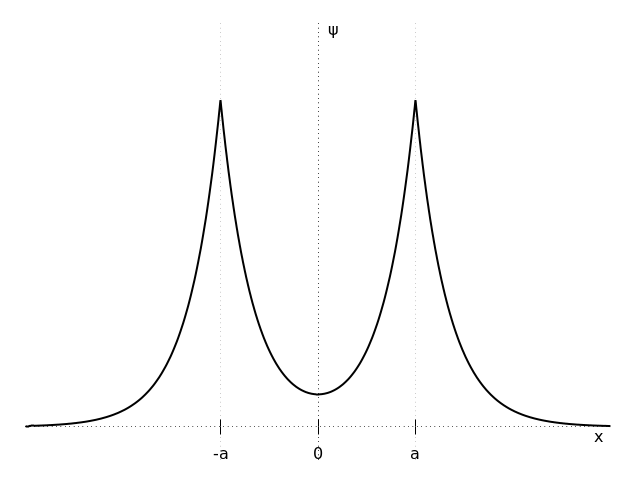
\includegraphics[width=\textwidth]{even.png}
    \caption{Even.}
  \end{subfigure}
  \begin{subfigure}[h]{0.48\textwidth}
    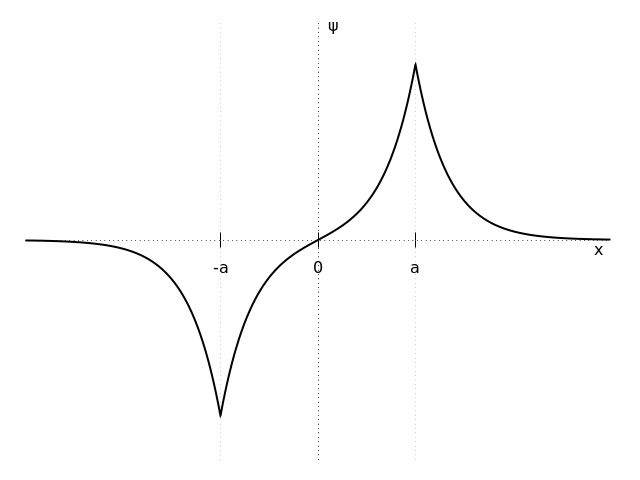
\includegraphics[width=\textwidth]{odd.png}
    \caption{Odd.}
  \end{subfigure}
  \caption{Wave functions of bound states.}
\end{figure}

\begin{figure}
  \centering
  \begin{subfigure}[h]{0.48\textwidth}
    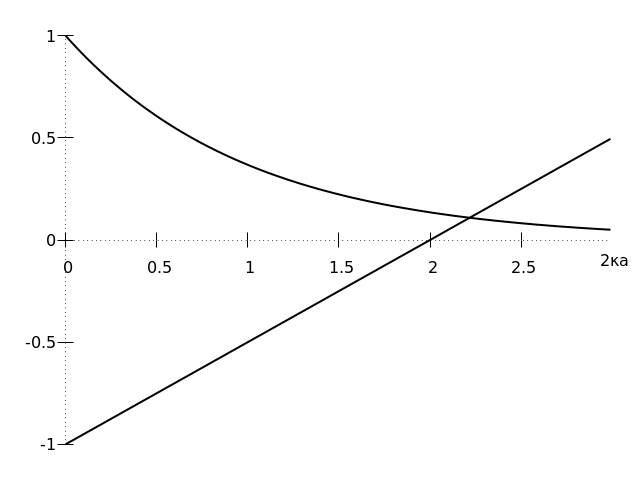
\includegraphics[width=\textwidth]{even_solution.png}
    \caption{Even eigenstate ($ak-1=e^{-2ka}$).}
  \end{subfigure}
  \begin{subfigure}[h]{0.48\textwidth}
    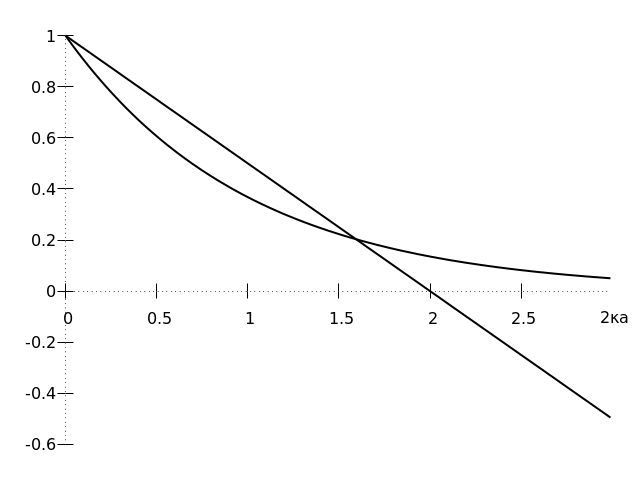
\includegraphics[width=\textwidth]{odd_solution.png}
    \caption{Odd eigenstate ($1-ak=e^{-2ka}$).}
  \end{subfigure}
  \caption{Graphical solutions to transcendental equations (double delta function potential).}
\end{figure}

\begin{figure}[!htb]
  \centering
  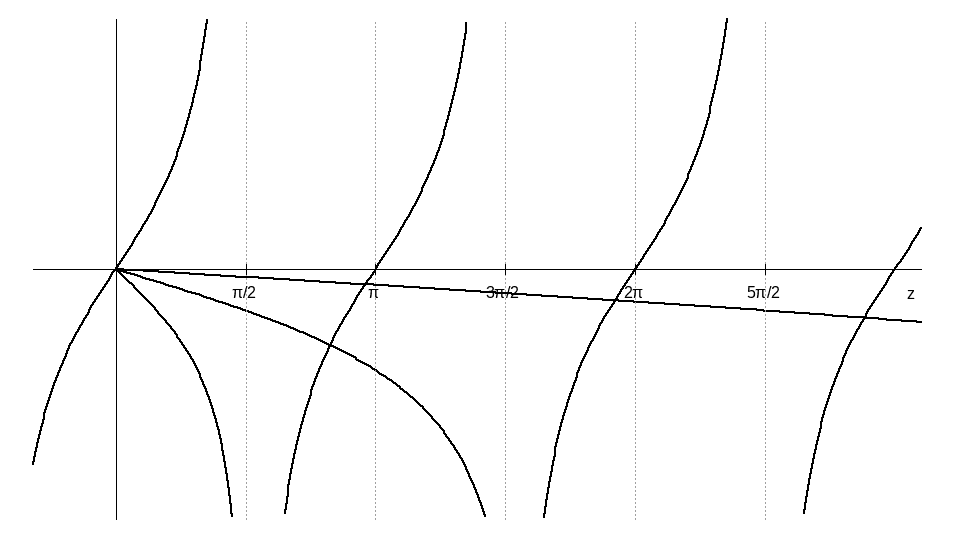
\includegraphics[width=0.7\textwidth]{odd_states.png}
  \caption{Graphical solution to equation $\tan{z}=-[(\frac{z_0}{z})^2-1]^{-\frac{1}{2}}$.}
\end{figure}

\section*{Scattering state wave amplitudes (in terms of A)}

$$B=-{{A\,e^{4\,i\,a\,k}\,\left(q^2-2\,i\,k\,q\right)+A\,\left(-q^2-2
 \,i\,k\,q\right)}\over{e^{6\,i\,a\,k}\,q^2+e^{2\,i\,a\,k}\,\left(-q^
 2-4\,i\,k\,q+4\,k^2\right)}}$$

$$C=-{{A\,\left(2\,i\,k\,q-4\,k^2\right)}\over{e^{4\,i\,a\,k}\,q^2-q^
 2-4\,i\,k\,q+4\,k^2}}$$

$$D={{2\,i\,A\,k\,e^{2\,i\,a\,k}\,q}\over{e^{4\,i\,a\,k}\,q^2-q^2-4\,
 i\,k\,q+4\,k^2}}$$

$$F={{4\,A\,k^2}\over{e^{4\,i\,a\,k}\,q^2-q^2-4\,i\,k\,q+4\,k^2}}$$

\section*{Computer math}

\lstinputlisting[language=Maxima]{hw4.max}

\end{document}
